\section{Method}
\label{sec:method}

\begin{figure}
	\center
	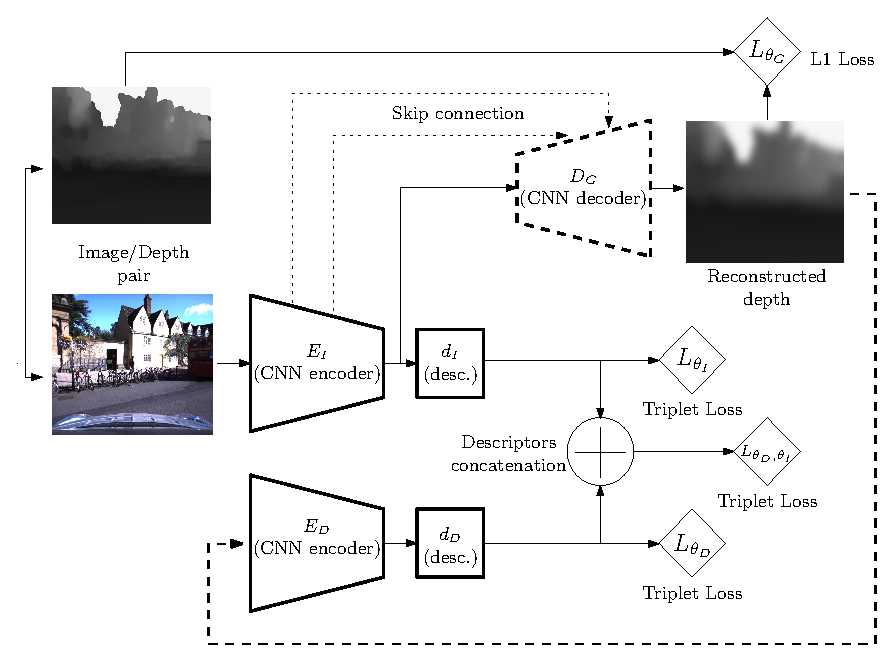
\includegraphics[width=\linewidth]{vect/our_method-inv}
	\caption{\label{fig:our_method} \textbf{Image descriptors training with auxiliary depth data:} two encoders are used for extracting deep features map from the main image modality and the auxiliary reconstructed depth map (inferred from our deep decoder). These features are used to create intermediate descriptors that are finally concatenated in one final image descriptor.}
\end{figure}

\begin{figure}
	\center
	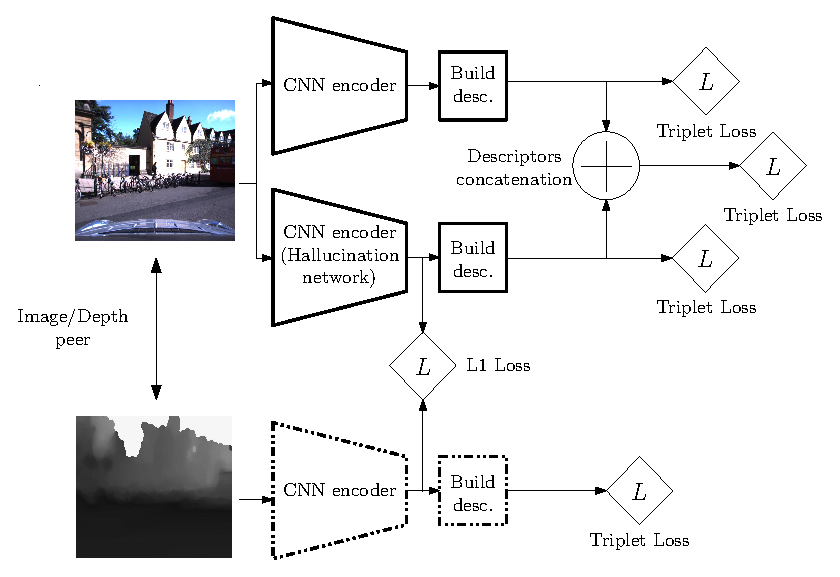
\includegraphics[width=\linewidth]{vect/hall_method-inv}
	\caption{\label{fig:hall_method} \textbf{Hallucination network for image descriptors learning:} we train an hallucination network, inspired from~\cite{Hoffman2016}, for the task of global image description. Unlike the proposed method (see figure~\ref{fig:our_method}), hallucination network reproduces feature maps that would have been obtained by a network trained with depth map rather than the deep map itself.}
\end{figure}

\subsection{Overview}
\label{subsec:overview}
We design a new global image description for the task of image-based localization. We first extract dense feature maps from an input image with a convolutional neural network encoder ($E_I$). These feature maps are subsequently used to build a compact representation of the scene ($d_I$). State-of-the-art features aggregation methods can be used to construct the image descriptor, such as MAC~\cite{Radenovic2017} or NetVLAD~\cite{Arandjelovic2017}. We enhance this standard image descriptor with side depth map information that is only available during the training process. To do so, a deep fully convolutional neural network decoder ($D_G$) is used to reconstruct the corresponding depth map according to the input image. The reconstructed depth is then used to extract a global depth map descriptor. We follow the same procedure used before: we extract deep feature maps with an encoder ($E_D$) before building the descriptor ($d_D$). Finally, the image descriptor $d_I$ and the depth map descriptor $d_D$ are concatenated into a single global descriptor. Figure~\ref{fig:our_method} summarizes the whole process of our method. Once trained with geometric and radiometric information, the proposed method is used on images only, to create a descriptor tuned for image localization.

\subsection{Training routine}
\label{subsec:training}
Trainable parameters are $\theta_{I}$ the weights of encoder and descriptor $\{E_I, d_I\}$, $\theta_{D}$ the weights of the encoder and descriptor $\{E_D, d_D\}$ and $\theta_{G}$ the weights of the decoder used for depth map generation. 

For training our system, we follow standard procedure of descriptor learning based on triplet margin losses~\cite{Arandjelovic2017}. A triplet $\{q_{im}, q_{im}^+, q_{im}^-\}$ is composed of an anchor image $q_{im}$, a positive example $q_{im}^+$ representing the same scene as the anchor and an unrelated negative example $q_{im}^-$.
The first triplet loss acting on $\{E_I, d_I\}$ is:
\begin{multline}
	\label{eq:triplet_loss}
	L_{\theta_{I}} = max\left(0, \lambda + \norm{f_{\theta_{I}}(q_{im}) - f_{\theta_{I}}(q_{im}^+)}_2  \right. \\	
	\left. - \norm{f_{\theta_{I}}(q_{im}) - f_{\theta_{I}}(q_{im}^-)}_2 \right),
\end{multline}
where $f_{\theta_{I}}(x_{im})$ is the global descriptor of image $x_{im}$ and $\lambda$ an hyper-parameter controlling the margin between positive and negative examples. $f_{\theta_{I}}$ can be written as:
\begin{equation}
	\label{eq:desc_details}
	f_{\theta_{I}}(x_{im}) = d_I(E_I(x_{im})),
\end{equation}
where $E_I(x_{im})$ represents the deep feature maps extracted by the decoder and $d_I$ the function used to build the final descriptor from the feature.

We train the depth map encoder and descriptor $\{E_D, d_D\}$ in a same manner, equation~(\ref{eq:triplet_loss}) becoming:
\begin{multline}
	\label{eq:depth_triplet_loss}
	L_{\theta_{D}}  = max\left(0, \lambda + \norm{f_{\theta_{D}}(\hat{q}_{depth}) - f_{\theta_{D}}(\hat{q}_{depth}^+))}_2  \right. \\	
	\left. - \norm{f_{\theta_{D}}(\hat{q}_{depth}) - f_{\theta_{D}}(\hat{q}_{depth}^-)}_2 \right),
\end{multline}
where $f_{\theta_{D}}(x_{depth})$ is the global descriptor of depth map $x_{depth}$ and $\hat{x}_{depth}$ is the reconstructed depth map of image $x_{im}$ by the decoder $D_G$:
\begin{equation}
	\label{eq:generator}
	\hat{x}_{depth} = D_G(E_I(x_{im})).
\end{equation}
Decoder $D_G$ uses the deep representation of image $x_{im}$ computed by encoder $E_I$ in order to reconstruct the scene geometry. Notice that even if the encoder $E_I$ is not especially trained for depth map reconstruction, its intern representation is rich enough to be used by the decoder $D_G$ for the task of depth map inference. We choose to use the features already computed by the first encoder $E_I$ instead of introducing another encoder for saving computational resources.

The final image descriptor is trained with the following loss:
\begin{multline}
	\label{eq:cat_triplet_loss}
	L_{\theta_{I},\theta_{D}} = max\left(0, \lambda + \norm{F_{\theta_{I},\theta_{D}}(q_{im}) - F_{\theta_{I},\theta_{D}}(q_{im}^+)}_2  \right. \\	
	\left. - \norm{F_{\theta_{I},\theta_{D}}(q_{im}) - F_{\theta_{I},\theta_{D}}(q_{im}^-)}_2 \right),
\end{multline}
where $F_{\theta_{I},\theta_{D}}(x_{im})$ denotes the concatenation of image descriptor and depth map descriptor:
\begin{equation}
	\label{eq:cat_function}
	F_{\theta_{I},\theta_{D}}(x_{im}) = \left[ f_{\theta_{I}}(x_{im}), f_{\theta_{D}}(\hat{x}_{depth}) \right].
\end{equation}

In order to train the depth map generator, we use a simple $L_1$ loss function:
\begin{equation}
 \label{eq:l1_loss}
	L_{\theta_{G}} = \norm{x_{depth} - \hat{x}_{depth}}_{1}.
\end{equation}

The whole system is trained according to the following constraints:
\begin{align}
	\left( \theta_{I}, \theta_{D} \right) & := arg\,\underset{\theta_{I}, \theta_{D}}{min} \left[ L_{\theta_{I}} + L_{\theta_{D}} + L_{\theta_{I},\theta_{D}} \right], \label{eq:sys_optimization_1} \\ 	
	\left( \theta_{G} \right) & := arg\,\underset{\theta_{G}}{min} \left[ L_{\theta_{G}} \right]. 	\label{eq:sys_optimization_2}
\end{align}

We use two different optimizers: one updating $\theta_{I}$ and $\theta_{D}$ weights regarding constraint~(\ref{eq:sys_optimization_1}) and the other updating $\theta_{G}$ weights regarding constraint~(\ref{eq:sys_optimization_2}). Because decoder $D_G$ relies on feature maps computed by encoder $E_I$ (see equation~\ref{eq:generator}), at each optimization step on $\theta_{I}$ we need to update decoder weights $\theta_{G}$ to take in account possible changes in the image features. We finally train our entire system, by alternating between the optimization of weights $\{\theta_{I}, \theta_{D}\}$ and $\{\theta_G\}$ until convergence.

\subsection{Hallucination network for image description}
\label{subsec:hall}
We compare our proposal with a state-of-the-art approach that is capable of training a system with side information, named hallucination network~\cite{Hoffman2016}. Hallucination network is originally designed for object detection and classification in an image. We adapt the work of~\cite{Hoffman2016} to create an image descriptor system that benefits from depth map side modality during training. Like our proposal, the trained hallucination network is used on image only and produce a global descriptor for image localization. The system is presented in figure~\ref{fig:hall_method}. The main difference with our proposal is that the hallucination network reproduces feature maps that would have been obtained by a network trained with depth map rather than the deep map itself. We refer readers to~\cite{Hoffman2016} for more information about the hallucination network.

One advantage of the hallucination network over our proposal is that it does not require a decoder network, resulting on a architecture lighter than ours. However, it needs a pre-training step, where image encoder and depth map encoder are trained separately from each other before a final optimization step with the hallucination part of the system. Our system do not need such initialization. Training the hallucination network requires more complex data than the proposed method. Indeed, it needs to gather triplets of \textit{\{image, depth map\}} pairs, which require to know the absolute position of the data~\cite{Arandjelovic2017,Liu2018}, or to use costly algorithms like Structure from Motion (SfM)~\cite{Godard2017,Radenovic2017,Kim2017a}. 

One advantage of our method over the hallucination approach is that we have two unrelated objectives during training: learning a efficient image representation for localization and learning how to reconstruct scene geometry from an image. It means we can train several parts of our system separately, with different source of data. Especially, we can improve the scene geometry reconstruction task with non localized \textit{\{image, depth map\}} pairs. These weakly annotated data are easier to gather than triplet, as we only need calibrated system capable of sensing radiometric and geometric modalities at the same time. We will show in practice how this can be exploited to fine tune the decoder part to deal with complex localization scenarios in part~\ref{subsec:results}.

